\documentclass[12pt]{article}
\usepackage[margin=1in]{geometry}
\usepackage{blindtext}
\usepackage{hyperref}
\usepackage{amsmath,epsfig}
\usepackage{amsfonts}
\usepackage[T1]{fontenc}
\usepackage{titling}
\usepackage{commath}
\usepackage{mathtools}
\usepackage{tabu}
\usepackage{booktabs}
\usepackage{bm}
\usepackage{xfrac}
\usepackage{listings}
\usepackage{float}
\newcommand{\RR}{\mathbb{R}}
\DeclarePairedDelimiter\ip{\langle }{\rangle}
\DeclareMathOperator{\proj}{proj}
\usepackage{subcaption}
\usepackage{graphicx}
\usepackage{tikz}
\usepackage{float}
\usepackage{subcaption}
\usepackage[backend=biber,style=authoryear]{biblatex}
\addbibresource{references.bib}

\usetikzlibrary{quotes, angles, intersections}
\setlength{\droptitle}{-10em}
\title{Final report draft}
\author{Jonathan Hayase\and Anqi He}
\begin{document}
\maketitle
\begin{abstract}\noindent
This paper presents the physical and mathematical theories behind a Monte Carlo ray tracer as well as the implementation of several importance sampling techniques. The rendered ray-tracing images are compared quantitatively with the converged image to demonstrate the difference in convergence rate between using uniform sampling and importance sampling approaches. The paper concludes with a summary of the results and discussion of future work.
\end{abstract}

\section{Introduction}
Ray tracing is a rendering technique for generating digital images by simulating how light would interact with the objects in the virtual scene. When a ray of light bounces off a surface, new rays of light are created, the ray tracer calculates all of the rays on a path. \\
\begin{figure}[ht]
  \centering
    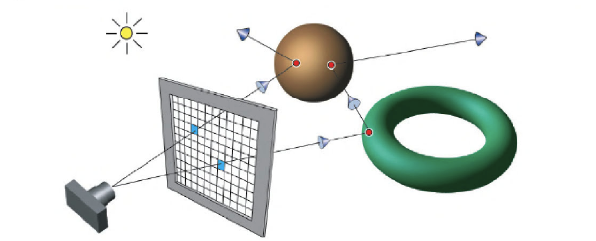
\includegraphics[width=0.5\textwidth]{figure1.png}
    \caption{Ray tracing}
\end{figure}
Forward ray tracing is a method that can most accurately determine the coloring of each object. It follows light particles from the light source to the objects and calculates the rays of light that arrive at the eye. However, realistically only a paltry number of rays would end up at the viewer's eyes, which makes this method highly inefficient to implement in practice.\\\\
To make the ray tracer more efficient, the method of backward ray tracing is implemented in this project. In backward ray tracing, the ray is created at the viewer's eye, the first object this ray arrives at will be visible to the viewer. The ray tracer follows this ray and as it bounces in the scene, and calculates the coloring of the particular point in the view plane where the ray was originally created. Given Helmholtz reciprocity principle, when the light interacts with a surface, the incoming and outgoing light can be considered as reversal of each other. Hence in ray tracing applications, these two ray tracing methods produce equivalent outcome. The diagrams below illustrate the two ray tracing approaches. \\
 \begin{figure}[H]
      \centering
      \begin{tikzpicture}
        \filldraw[color = gray!40, draw=black] (-1.4,-0.4) -- (-0.6,-0.5) -- (-0.6,0.5) -- (-1.4, 0.4) -- cycle;
        \draw[thick] (-1,0) -- (-3,-1) node[midway, below] {\(\bm{\omega_i}\)};
        \draw[->] (-1,0)  --(-3,1.2) node[midway, above] {\(\bm{\omega_o}\)};
        \draw[->] (-1,0)  --(-3,1);
        \draw[->] (-1,0)  --(-3,0.8);
      \end{tikzpicture}
      \caption{\textbf{Forward path tracing}, i.e. trace ``light rays'' from lights to eye.}
    \end{figure}
    
    \begin{figure}[H]
      \centering
      \begin{tikzpicture}
        \filldraw[color = gray!40, draw=black] (-1.4,-0.4) -- (-0.6,-0.5) -- (-0.6,0.5) -- (-1.4, 0.4) -- cycle;
        \draw[->] (-1,0) -- (-3,-0.8);
        \draw[->] (-1,0) -- (-3,-1); 
        \draw[->] (-1,0) -- (-3,-1.2) node[midway, below] {\(\bm{\omega_i}\)};
        \draw[thick] (-1,0)  --(-3,1) node[midway, above] {\(\bm{\omega_o}\)};
      \end{tikzpicture}
      \caption{\textbf{Backward path tracing}, i.e. trace ``eye rays'' from eye to lights.}
    \end{figure}

\noindent The goal of this project is to quantitatively compare the results of using importance sampling and uniform sampling ray tracing application. The a ray of light bounces at a surface, the uniform sampling method picks the next ray of a random direction in the light path, whereas importance sampling automatically selects a direction based on how much it will contribute to the radiance, hence the insignificant directions are selected less often. In this project, we compare the convergence rate under uniform sampling and importance sampling methods by plotting the Root Mean Squared Error between the converged matrix and rendered matrices at different number of samples.
\newline
    
\section{Theory}
\subsection{Introduction: the rendering equation}
The physical basis for all raytracers is the rendering equation, which can be written as\footnote{cite this}
\[L_{o}(\mathbf x, \bm {\omega_{o}}, \lambda, t) = L_{e}(\mathbf x, \bm{\omega_o}, \lambda, t) + \int_\Omega f_s(\mathbf x, \bm{\omega_i}, \bm{\omega_o}, \lambda, t)L_i(\mathbf x, \bm{\omega_i}, \lambda, t)\ip{\bm n, \bm{\omega_i}} \dif \bm{\omega_i}\]

where
\begin{center}
  \begin{tabu}{ll}
    \(L_{o}\) is the outbound radiance & \(\bm{\omega_o}\) is the outbound radiance direction\\
    \(L_{i}\) is the inbound radiance & \(\bm{\omega_i}\) is inbound radiance direction\\
    \(L_{e}\) is the emission radiance & \(\mathbf x\) is a point in space\\
    \(f_s\) bidirectional scattering distribution function & \(\lambda\) is the spectral wavelength\\
    \(\Omega\) is the unit hemisphere around \(\bm n\) & \(\bm n\) is the surface normal at \(\mathbf x\).
  \end{tabu}
\end{center}
Since we are rendering only still images, we can ignore the dependence on time, yielding
\[L_{o}(\mathbf x, \bm {\omega_{o}}, \lambda) = L_{e}(\mathbf x, \bm{\omega_o}, \lambda) + \int_\Omega f_s(\mathbf x, \bm{\omega_i}, \bm{\omega_o}, \lambda)L_i(\mathbf x, \bm{\omega_i}, \lambda)\ip{\bm n, \bm{\omega_i}} \dif \bm{\omega_i}.\]

Solving the rendering equation for a given set of objects is the main task in accurate rendering algorithms.
However, the equation is recursive, as the outbound radiance at one point may become the inbound radiance at another.
Thus, a realistic solution to the rendering equation requires integrating over all possible paths light may take within a scene.
For scenes of any reasonable complexity, this produces a system that is too complex to be solved analytically.

Therefore, it is appropriate to compute an approximate solution to the rendering equation using Monte Carlo methods.
Raytracers operate by explicitly tracing light paths through the scene.
By averaging over enough paths, they can produce a highly accurate approximate solutions to the rendering equation.
In this paper, we have chosen to implement forward path tracing.
In this method, light rays start at the observer and bounce through the scene until they encounter a light.
This is the opposite of the normal intuition involving light, as photons themselves travel from light sources to the observer.
However, due to Helmholtz reciprocity, the result is the same.
The advantage of this method over tracing light from light sources to the observer is that it is easier to control the sampling distribution of rays with respect to the observer, which generally leads to more straightforward convergence.

The path tracing algorithm can be described by the following highly simplified psuedo code
\begin{lstlisting}
def radiance(ray):
    if the recursion depth is above a certain threshold:
        return black
    if the ray does not hit an object in the scene:
        return black
    let obj be the object hit by the ray
    let i be a randomly sampled input ray
    let r be radiance(i)
    add the emission of obj to r
    calculate the spectral output given ray, i, and r
\end{lstlisting}
Accordingly, the focus of this paper will be on intelligent sampling the input ray \(\bm i\) from this description.

\subsection{Calculating reflected light}
\subsubsection{Defining the bidirectional scattering distribution function}
Until this point, the details of the interaction of light at the surface of an object have not been discussed.
The optical properties of a material are defined exclusively by its bidirectional scattering distribution function or BSDF, notated \(f_s\).
The BSDF is a function of four parameters:
\begin{enumerate}
\item \(\mathbf x\) the point in space at which the light hit the object
\item \(\bm{\omega_o}\) the outbound radiance direction
\item \(\bm{\omega_i}\) the inbound radiance direction
\item \(\lambda\) the wavelength
\end{enumerate}
We will operate under the assumption that the BSDF remains uniform across the surface of an object.
Thus, in the context of a specific material, there is no dependence on \(\mathbf x\).
The output of the BSDF is the proportion of light reflected according to the given parameters.

Physical materials often have the property that their BSDF is invariant as \(\bm{\omega_o}\) and \(\bm{\omega_i}\) are both rotated about the surface normal \(\bm n\).
This is known as isotropy, and in this paper we will assume that all materials are isotropic.
Therefore in practice, it is convenient to re-parameterize the BSDF in terms relative to the surface normal \(\bm n\).
\begin{figure}[H]
  \begin{subfigure}[b]{0.5\textwidth}
    \centering
    \begin{tikzpicture}
      \filldraw[color = gray!40, draw=black] (-1,-1) -- (1,-1) -- (1,1) -- (-1, 1) -- cycle;
      \draw[->] (0,0) coordinate (o) -- (-1.3,1.1) coordinate (wi) node[pos=1.15] {\(\bm{\omega_i}\)};
      \draw[->] (0,0)  --(1.4,1) coordinate (wo) node [pos=1.15] {\(\bm{\omega_o}\)};
      \node (0,0) [below] {\(\bm n\)};
      \filldraw (0,0) circle (1pt);
      \draw pic["$\phi_\Delta$",draw=black,angle eccentricity=2,angle radius=0.3cm] {angle=wo--o--wi};
    \end{tikzpicture}
    \caption{Definition of \(\phi_\Delta\).}
  \end{subfigure}
  %
  \begin{subfigure}[b]{0.5\textwidth}
    \centering
    \begin{tikzpicture}
      \filldraw[color = gray!40, draw=black] (-1.5,-0.3) -- (1.5,-0.3) -- (1,0.3) -- (-1, 0.3) -- cycle;
      \draw[->] (0,0) coordinate (o) -- (-1.2,1.2) coordinate (wi) node [pos=1.15] {\(\bm{\omega_i}\)};
      \draw[->] (0,0)  --(1.2,1.2) coordinate (wo) node [pos=1.15] {\(\bm{\omega_o}\)};
      \draw[->] (0,0) -- (0, 1.5) coordinate (n) node [above] {\(\bm n\)};
      \filldraw (0,0) circle (1pt);
      \draw pic["$\theta_{\bm o}$",draw=black,angle eccentricity=1.4,angle radius=0.8cm] {angle=n--o--wi};
      \draw pic["$\theta_{\bm i}$",draw=black,angle eccentricity=1.4,angle radius=0.8cm] {angle=wo--o--n};
    \end{tikzpicture}
    \caption{Definition of \(\theta_{\bm o}\) and \(\theta_{\bm i}\).}
  \end{subfigure}
  \caption{Spherical reparameterization about \(\bm n\).}
\end{figure}
Geometrically, these parameters are defined as
\begin{align*}
  \theta_{\bm i} &= \cos^{-1} \ip{\bm{\omega_i}, \bm n}\\
  \theta_{\bm o} &= \cos^{-1} \ip{\bm{\omega_o}, \bm n}\\
  \phi_\Delta &= \cos^{-1}\del{\frac{\del{\bm{\omega_o} - \proj_{\bm n} \bm{\omega_o}} \cdot \del{\bm{\omega_i} - \proj_{\bm n} \bm{\omega_i}}}{\norm{\bm{\omega_o} - \proj_{\bm n} \bm{\omega_o}} \cdot \norm{\bm{\omega_i} - \proj_{\bm n} \bm{\omega_i}}}}.
\end{align*}
Thus, \(f_s\) is a function of \(\theta_{\bm i}\), \(\theta_{\bm o}\), and \(\phi_\Delta\) where
\begin{enumerate}
\item \(\theta_{\bm i}\) is the angle off the normal of \(\bm{\omega_i}\)
\item \(\theta_{\bm o}\) is the angle off the normal of \(\bm{\omega_o}\)
\item \(\phi_\Delta\) is the angle between \(\bm{\omega_i}\) and \(\bm{\omega_o}\) about the axis of rotation defined by \(\bm n\)
\end{enumerate}

\subsubsection{Integrating the BSDF with importance sampling}
Returning to the rendering equation, we see that in general while path tracing we have no knowledge of the distribution of \(L_i(\mathbf x, \bm{\omega_i}, \lambda, t)\).
However, since we know the material properties, we have complete knowledge of the distribution of \(f_s(\mathbf x, \bm{\omega_i}, \bm{\omega_o}, \lambda, t)\ip{\bm n, \bm{\omega_i}} = f_s(\theta_{\bm i}, \theta_{\bm o}, \phi_\Delta)\cos \theta_{\bm i}\).
Therefore, we can use the knowledge of the BSDF distribution to perform importance sampling of the light paths while path tracing, allowing the approximation to converge faster.

\subsection{Example: Lambertian Diffuse BSDF}
\subsubsection{BSDF description}
Perhaps the simplest possible BSDF is the Lambertian Diffuse BSDF, which describes an ideal diffuse surface.
\[f_s(\theta_{\bm i}, \theta_{\bm o}, \phi_\Delta) = \frac{\rho_d}{\pi}\]
where \(\rho_d \in \intcc{0,1}\) is the albedo, or normal reflectance of the material.
Thus, the Lambertian BSDF describes completely uniform scattering of light in all directions.
In general, we will assume that diffuse surfaces do not emit light.
Therefore, substitution into the rendering equation yields
\begin{align*}
  L_{o}(\mathbf x, \bm {\omega_{o}}, \lambda)
  &= \rho_d \int_\Omega \frac{1}{\pi} L_i(\mathbf x, \bm{\omega_i}, \lambda)\cos\theta_{\bm i} \dif \bm{\omega_i}\\
  &= \rho_d \int_0^{2\pi}\int_0^{\sfrac{\pi}{2}} \frac{1}{\pi} L_i(\mathbf x, \bm{\omega_i}, \lambda)\cos\theta_{\bm i} \sin\theta_{\bm i}\dif \theta_{\bm i} \dif \phi_\Delta.
\end{align*}
Thus, we are interested in importance sampling with respect to the PDF
\[P(\theta_{\bm i}, \phi_\Delta) = \frac{1}{\pi}\cos \theta_{\bm i}\sin \theta_{\bm i} = \frac{\sin 2\theta_{\bm i}}{2\pi}\]
\subsubsection{Importance sampling derivation}
Since the BSDF is isotropic, we can ignore \(\phi_\Delta\) completely, and sample purely with respect to \(\theta_{\bm i}\).
Therefore, we can define the PDF with respect to \(\theta_{\bm i}\) only as
\[P(\theta_{\bm i}) = \int_0^{2\pi} P(\theta_{\bm i}, \phi)\dif \phi = \int_0^{2\pi} \frac{\sin 2\theta_{\bm i}}{2\pi} \dif \phi = \sin 2\theta_{\bm i}\]
Now, we can find the CDF of the distribution like so
\begin{align*}
  F(\theta_{\bm i})
  &= \int_0^{\theta_{\bm i}} P(\theta) \dif \theta && \text{definition of CDF}\\
  &= \int_0^{\theta_{\bm i}} \sin 2\theta \dif \theta && \text{substitute}\\
  &= -\frac{1}{2}\cos 2\theta_{\bm i} + \frac{1}{2} && \text{integrate}\\
  &= \sin^2 \theta_{\bm i} && \text{trig identity}
\end{align*}
Now, letting \(\xi_\theta \sim \mathcal{U}(0, 1)\) and inverting the CDF with respect to \(\xi_\theta\) yields
\begin{align*}
  \xi_\theta &= F(\theta_{\bm i}) && \text{setup for CDF inversion}\\
  \xi_\theta &= \sin^2 \theta_{\bm i} && \text{substitute}\\
  \theta_{\bm i} &= \sin^{-1}\sqrt{\xi_\theta} && \text{solve for \(\theta_{\bm i}\)}
\end{align*}
And finally from our isotropy assumption we draw \(\xi_\phi \sim \mathcal{U}(0, 1)\).
Then
\[\phi_\Delta = 2\pi\xi_\phi .\]

\subsection{Example: Trowbridge-Reitz Microfacet Glossy BSDF}

\subsubsection{Ideal mirrors}

The direct opposite of a ideal diffuse surface is a ideal reflecting surface, or mirror.
While the BSDF of an ideal diffuse surface is uniform, the BSDF for an ideal mirror is a double Dirac delta function
\[f_s(\theta_{\bm i}, \theta_{\bm o}, \phi_\Delta) = \rho_s \delta(\theta_{\bm i} - \theta_{\bm o})\delta(\phi_\Delta + \pi).\]
where \(\rho_s \in \intcc{0, 1}\) is the specular albedo.
Thus, no sampling of the BSDF is needed, as \(\bm{\omega_i}\) is uniquely determined by
\[\bm{\omega_i} = 2\abs{\ip{\bm{\omega_o}, \bm n}}\bm n-  \bm{\omega_o}.\]
However in practice very few real materials can be accurately approximated by ideal reflectors.
Therefore, there exist several modifications to the BSDF which yield more accurate results.

\subsubsection{Fresnel conditions}

In general, glossy surfaces do not reflect all incident light.
In the case of dielectric materials, some light may be transmitted internally.
In the case of conductors, incident light may be absorbed and converted into heat.
This phenomenon is described by the Fresnel term \(F(\theta_{\bm i})\) which calculates the fraction of reflected light as a function of the inbound angle.
It takes the form\footnote{Cite this.}
\[F(\theta_{\bm i}) = \frac{r_{\parallel}^2 + r_{\perp}^2}{2}\]
where
\begin{align*}
  r_{\parallel} &= \norm{\frac{n_1 \cos \theta_{\bm i} - n_2 \sqrt{1 - \del{\frac{n_1}{n_2}\sin \theta_{\bm i}}^2}}{n_1 \cos \theta_{\bm i} + n_2 \sqrt{1 - \del{\frac{n_1}{n_2}\sin \theta_{\bm i}}^2}}}\\
  r_{\perp} &= \norm{\frac{n_1 \sqrt{1 - \del{\frac{n_1}{n_2}\sin \theta_{\bm i}}^2} - n_2\cos \theta_{\bm i}}{n_1 \sqrt{1 - \del{\frac{n_1}{n_2}\sin \theta_{\bm i}}^2} + n_2 \cos \theta_{\bm i}}}
\end{align*}
and
\begin{enumerate}
\item \(n_1\) is the complex index of refraction of the external medium
\item \(n_2\) is the complex index of refraction of the external medium
\end{enumerate}
In our case, we will make the assumption that the metal is surrounded by air, so \(n_1 \approx 1\).
This allows is to simplify to
\begin{align*}
  r_{\parallel} &= \norm{\frac{\cos \theta_{\bm i} - n_2 \sqrt{1 - \del{\frac{1}{n_2}\sin \theta_{\bm i}}^2}}{\cos \theta_{\bm i} + n_2 \sqrt{1 - \del{\frac{1}{n_2}\sin \theta_{\bm i}}^2}}}\\
  r_{\perp} &= \norm{\frac{\sqrt{1 - \del{\frac{1}{n_2}\sin \theta_{\bm i}}^2} - n_2\cos \theta_{\bm i}}{\sqrt{1 - \del{\frac{1}{n_2}\sin \theta_{\bm i}}^2} + n_2 \cos \theta_{\bm i}}}.
\end{align*}
The index of refraction of metals is canonically represented as \(n_2 = \eta + i\kappa\) where \(\eta\) is the traditional refractive index, and \(\kappa\) is the extinction coefficient.
Substituting this yields
\begin{align*}
  r_{\parallel} &= \norm{\frac{\cos \theta_{\bm i} - \del{\eta + i\kappa} \sqrt{1 - \del{\frac{1}{\del{\eta + i\kappa}}\sin \theta_{\bm i}}^2}}{\cos \theta_{\bm i} + \del{\eta + i\kappa} \sqrt{1 - \del{\frac{1}{\del{\eta + i\kappa}}\sin \theta_{\bm i}}^2}}}\\
  r_{\perp} &= \norm{\frac{\sqrt{1 - \del{\frac{1}{\del{\eta + i\kappa}}\sin \theta_{\bm i}}^2} - \del{\eta + i\kappa}\cos \theta_{\bm i}}{\sqrt{1 - \del{\frac{1}{\del{\eta + i\kappa}}\sin \theta_{\bm i}}^2} + \del{\eta + i\kappa} \cos \theta_{\bm i}}}.
\end{align*}
Now, we make the simplifying assumption that \(\eta^2 + \kappa^2 \gg 1\). Then we have
\[\sqrt{1 - \del{\frac{1}{\del{\eta + i\kappa}}\sin \theta_{\bm i}}^2} \approx 1\]
This allows us to approximate the terms by
\begin{align*}
  r_{\parallel}^2 &\approx \norm{\frac{\cos \theta_{\bm i} - \del{\eta + i\kappa}}{\cos \theta_{\bm i} + \del{\eta + i\kappa}}}^2\\
  r_{\perp}^2 &\approx \norm{\frac{1 - \del{\eta + i\kappa}\cos \theta_{\bm i}}{1 + \del{\eta + i\kappa} \cos \theta_{\bm i}}}^2.
\end{align*}
We can then expand the complex norm like so
\begin{align*}
  r_{\parallel}^2 &= \frac{\del{\cos \theta_{\bm i} - \del{\eta + i\kappa}}\del{\cos \theta_{\bm i} - \del{\eta - i\kappa}}}{\del{\cos \theta_{\bm i} + \del{\eta + i\kappa}}\del{\cos \theta_{\bm i} + \del{\eta - i\kappa}}}\\
  r_{\perp}^2 &= \frac{\del{1 - \del{\eta + i\kappa}\cos \theta_{\bm i}}\del{1 - \del{\eta - i\kappa}\cos \theta_{\bm i}}}{\del{1 + \del{\eta + i\kappa} \cos \theta_{\bm i}}\del{1 + \del{\eta - i\kappa} \cos \theta_{\bm i}}}.
\end{align*}
Simplifying yields
\begin{align*}
  r_{\parallel}^2 &= \frac{\del{\eta^2 + \kappa^2}\cos^2 \theta_{\bm i} - 2\eta \cos \theta_{\bm i} + 1}{\del{\eta^2 + \kappa^2}\cos^2 \theta_{\bm i} + 2\eta \cos \theta_{\bm i} + 1}\\
  r_{\perp}^2 &= \frac{\del{\eta^2 + \kappa^2} - 2\eta \cos \theta_{\bm i} + \cos^2 \theta_{\bm i}}{\del{\eta^2 + \kappa^2} + 2\eta \cos \theta_{\bm i} + \cos^2 \theta_{\bm i}}\\
  F(\theta_{\bm i}) &= \frac{r_{\parallel}^2 + r_{\perp}^2}{2}.
\end{align*}

This is the Fresnel approximation we use in our raytracer.
Additionally, this is equivalent to the Fresnel approximation used in the PBRT raytracer.
The Fresnel term is then incorporated into the BSDF directly as
\[f_s(\theta_{\bm i}, \theta_{\bm o}, \phi_\Delta) = \rho_s \delta(\theta_{\bm i} - \theta_{\bm o})\delta(\phi_\Delta + \pi)F(\theta_{\bm i})\]

\subsubsection{Trowbridge-Reitz microfacet distribution}

In addition to changes in the amount of reflected light, many surfaces exhibit blurred reflection due to surface scattering.
This is due to microscopic variation in the surface.
Therefore, the surface can be though of as consisting many tiny facets, each of which acts as its own ideal reflector, called microfacets.
Many competing models for the distribution of orientations of the microfacet normals exist.
We have chosen to implement the Trowbridge-Reitz microfacet distribution, which was shown to produce visually accurate results in \footnote{cite EGSR07}.
It takes the form
\[D(\bm m) = \frac{\alpha^2 \chi^+(\ip{\bm m, \bm n})}{\pi\del{\del{\alpha^2 - 1}\cos^2 \theta_{\bm m} + 1}^2}.\]
where
\begin{enumerate}
\item \(D(\bm m)\) is the probability density of the microfacet distribution with normal vector \(\bm m\)
\item \(\chi^+(x)\) is the positive characteristic function, which is \(1\) if \(x>0\) and \(0\) otherwise
\item \(\theta_{\bm m}\) is the angle between the macrosurface normal \(\bm n\) and \(\bm m\)
\item \(\alpha > 0\) is the width parameter, which characterizes the amount of surface roughness.
\end{enumerate}
Note that, in the limiting case \(\alpha \to 0\), then if \(\bm m \neq \bm n\) we have
\begin{align*}
  \lim_{\alpha \to 0^+}D(\bm m)
  &= \lim_{\alpha \to 0^+}\frac{\alpha^2 \chi^+(\ip{\bm m, \bm n})}{\pi\del{\del{\alpha^2 - 1}\cos^2 \theta_{\bm m} + 1}^2}\\
  &= \frac{ \chi^+(\ip{\bm m, \bm n})}{\pi}\lim_{\alpha \to 0^+}\frac{\alpha^2}{\del{\del{\alpha^2 - 1}\cos^2 \theta_{\bm m} + 1}^2} && \text{simplify}\\
  &= 0
\end{align*}
Since \(\alpha^2\) goes to \(0\), but \(\del{\alpha^2 - 1}\cos^2 \theta_{\bm m} + 1\) must go to some positive number since \(0 \leq \cos\theta_{\bm m} < 1\).
On the other hand, if \(\bm m = \bm n\) then
\begin{align*}
  \lim_{\alpha \to 0}D(\bm m)
  &= \lim_{\alpha \to 0^+}\frac{\alpha^2}{\pi\del{\del{\alpha^2 - 1} + 1}^2} && \text{since \(\ip{\bm m, \bm n} = \cos \theta_{\bm m} = 1\)}\\
  &= \frac{1}{\pi}\lim_{\alpha \to 0^+}\frac{1}{\alpha^2} && \text{simplify}\\
  &= +\infty
\end{align*}
Thus, the Trowbridge-Reitz microfacet distribution reproduces the Dirac delta behavior of an ideal reflector in the limit \(\alpha \to 0\).

Note that the probability distribution describes the distribution of the normal vectors.
To make this useful, we must calculate the microfacet normal given \(\bm{\omega_i}\) and \(\bm{\omega_o}\).
Fortunately, this is easy to do when the microfacet is an ideal reflector.
The microfacet normal can solved for like so
\begin{align*}
  \bm{\omega_i} &= 2\abs{\ip{\bm{\omega_o}, \bm m}}\bm m-  \bm{\omega_o} && \text{ideal reflection formula}\\
  \bm m &= \frac{\bm{\omega_i} + \bm{\omega_o}}{2\abs{\ip{\bm{\omega_o}, \bm n}}} && \text{solve for \(\bm m\)}\\
  \bm m &= \frac{\bm{\omega_i} + \bm{\omega_o}}{\norm{\bm{\omega_i} + \bm{\omega_o}}} && \text{alternative normalization}
\end{align*}
Therefore, the microfacet distribution can be incorporated into the BSDF as
\[f_s(\theta_{\bm i}, \theta_{\bm o}, \phi_\Delta) = \rho_sF(\theta_{\bm i})D\del{\frac{\bm{\omega_i} + \bm{\omega_o}}{\norm{\bm{\omega_i} + \bm{\omega_o}}}}.\]

\subsubsection{Smith microfacet shadow masking}

Since it is physically reasonable to consider microfacets as being part of a continuous surface, then it is possible to model the surface in the neighborhood of a point as being defined by some height function \(z = f(x, y)\).
However, these microscopic differences in height will cause the surface micro geometry to cast shadows on itself, thus it is possible for a ray \( \bm r\) to intersect with multiple micro facets.
\begin{figure}[H]
  \centering
  \begin{tikzpicture}[domain=1:5,samples=200]
    \draw[name path=surface] plot (\x, {0.3*sin(6*\x r)});
    \draw[name path=ray,draw=none] (5,1) -- (1.4,-0.3);
    \draw[thick,name intersections={of=ray and surface}, ->](5,1)--(intersection-3);
    \draw[name intersections={of=ray and surface}, ->](intersection-3)--(1.4,-0.3);
  \end{tikzpicture}
  \caption{A ray intersecting with a micro surface multiple times.}
\end{figure}

To avoid double-counting, we must employ a corrective term.
This term is known as the shadow masking function, \(G(\bm{\omega_i}, \bm{\omega_o}, \bm m)\), which describes what proportion of the micro facets with normal \(\bm m\) are visible simultaneously from directions \(\bm{\omega_i}\) and \(\bm{\omega_o}\).
The Smith shadow masking function approximates \(G\) as the separable product two monodirectional masking terms
\[G(\bm{\omega_i}, \bm{\omega_o}, \bm m) = G_1(\bm{\omega_i}, \bm m)G_1(\bm{\omega_i}, \bm m)\]
The Smith shadow masking term is dependent on the microfacet distribution, \(D\).
For the Trowbridge-Reitz distribution, \(G_1\) takes the form \autocite{walter2007microfacet}
\[G_1(\bm v, \bm m) = \chi^2\del{\frac{\ip{\bm v, \bm m}}{\ip{\bm v, \bm n}}} \frac{2}{1 + \sqrt{1 + \alpha^2 \tan^2{\theta_{\bm v}}}}\]
where
\begin{enumerate}
\item \(\bm v\) is the viewing direction (may be either \(\bm{\omega_o}\) or \(\bm{\omega_i}\))
\item \(\theta_{\bm v}\) is the angle between the macrosurface normal \(\bm n\) and \(\bm m\).
\end{enumerate}
The Smith shadow masking correction is incorporated into the BSDF in the same way as the microfacet distribution function.
Thus the BSDF becomes
\[f_s(\theta_{\bm i}, \theta_{\bm o}, \phi_\Delta) = \rho_sF(\theta_{\bm i})D\del{\frac{\bm{\omega_i} + \bm{\omega_o}}{\norm{\bm{\omega_i} + \bm{\omega_o}}}}G\del{\bm{\omega_i}, \bm{\omega_o}, \frac{\bm{\omega_i} + \bm{\omega_o}}{\norm{\bm{\omega_i} + \bm{\omega_o}}}}.\]

\subsubsection{Importance sampling derivation}

Importance sampling is especially suitable for glossy surfaces, as the distribution of inbound light is highly nonuniform.
In fact, in the limit as \(\alpha \to 0\) we see that the distribution collapses towards a Dirac delta function.
However, sampling is not trivial as it was for ideal reflectors, as the light distribution caused by variation in the microfacet normals is complex.

In order to simplify our calculations, we will assume that \(D\) is the main contributor to the shape of the BSDF.
This allows us to sample in terms of the microfacet normal \(\bm m\).
To use this sampling we can transform from \(\bm{\omega_o}\) and \(\bm{\omega_i}\) to \(\bm m\) and back.

Recall the Trowbridge-Reitz microfacet distribution function
\[D(\bm m) = \frac{\alpha^2 \chi^+(\ip{\bm m, \bm n})}{\pi\del{\del{\alpha^2 - 1}\cos^2 \theta_{\bm m} + 1}^2}.\]
Substituting this into the rendering equation, and solving for \(\omega_i\) in terms of \(\bm m\) yields
\begin{align*}
  L_{o}(\mathbf x, \bm {\omega_{o}}, \lambda)
  &= \int_\Omega D(\bm m) L_i(\mathbf x, 2\abs{\ip{\bm{\omega_o}, \bm n}}\bm n-  \bm{\omega_o}, \lambda)\cos\theta_{\bm m} \dif \bm{m}\\
  &= \int_\Omega \frac{\alpha^2 \cos\theta_{\bm m} }{\pi\del{\del{\alpha^2 - 1}\cos^2 \theta_{\bm m} + 1}^2}\cdot L_i(\mathbf x, 2\abs{\ip{\bm{\omega_o}, \bm n}}\bm n-  \bm{\omega_o}, \lambda) \dif \bm{m}\\
  &= \int_0^{2\pi}\int_0^{\sfrac{\pi}{2}} \frac{\alpha^2 \cos\theta_{\bm m} \sin\theta_{\bm m}}{\pi\del{\del{\alpha^2 - 1}\cos^2 \theta_{\bm m} + 1}^2}\cdot L_i(\mathbf x, 2\abs{\ip{\bm{\omega_o}, \bm n}}\bm n-  \bm{\omega_o}, \lambda)\dif\theta_{\bm m}\dif\phi_\Delta\\
\end{align*}
Accordingly, we wish to sample the PDF
\[P_{\bm m}(\theta_{\bm m}, \phi_\Delta) = \frac{\alpha^2 \cos\theta_{\bm m} \sin\theta_{\bm m}}{\pi\del{\del{\alpha^2 - 1}\cos^2 \theta_{\bm m} + 1}^2} .\]
As in the Lambertian diffuse the BSDF is isotropic, we can ignore \(\phi_\Delta\) completely, and sample purely with respect to \(\theta_{\bm i}\).
Therefore, we can define the PDF with respect to \(\theta_{\bm i}\) only as
\[P_{\bm m}(\theta_{\bm m}) = \int_0^{2\pi}\frac{\alpha^2 \cos\theta_{\bm m} \sin\theta_{\bm m}}{\pi\del{\del{\alpha^2 - 1}\cos^2 \theta_{\bm m} + 1}^2}\dif\phi_\Delta = \frac{2\alpha^2 \cos\theta_{\bm m} \sin\theta_{\bm m}}{\del{\del{\alpha^2 - 1}\cos^2 \theta_{\bm m} + 1}^2}.\]
Next, we find the CDF of the distribution like so
\begin{align*}
  F_{\bm m}(\theta_{\bm m})
  &= \int_0^{\theta_{\bm m}} P(\theta)\dif\theta && \text{definition of CDF}\\
  &= \int_0^{\theta_{\bm m}} \frac{2\alpha^2 \cos\theta \sin\theta}{\del{\del{\alpha^2 - 1}\cos^2 \theta + 1}^2}\dif\theta && \text{substitute}\\
  &= \int_{\del{\alpha^2 - 1}\cos^20 + 1}^{\del{\alpha^2 - 1}\cos^2\theta_{\bm m} + 1} -\frac{\alpha^2}{\del{\alpha^2 - 1} u^2}\dif\theta && \begin{cases}
    \begin{aligned}
      u &= \del{\alpha^2 - 1}\cos^2\theta + 1\\
      \dif u &= -2\del{\alpha^2 - 1}\sin \theta \cos \theta \dif \theta
    \end{aligned}
  \end{cases} \\
  &= -\frac{\alpha^2}{\alpha^2 - 1} \int_{\alpha^2}^{\del{\alpha^2 - 1}\cos^2\theta_{\bm m} + 1} \frac{1}{u^2}\dif\theta && \text{simplify}\\
  &= -\frac{\alpha^2}{\alpha^2 - 1} \left[ -\frac{1}{u} \right]_{\alpha^2}^{\del{\alpha^2 - 1}\cos^2\theta_{\bm m} + 1} && \text{integrate}\\
  &= \frac{\alpha^2}{\alpha^2 - 1}  \del{\frac{1}{\del{\alpha^2 - 1}\cos^2\theta_{\bm m} + 1} - \frac{1}{\alpha^2}}  && \text{substitute}
\end{align*}
Now, letting \(\xi_\theta \sim \mathcal{U}(0, 1)\) and inverting the CDF with respect to \(\xi_\theta\) yields
\begin{align*}
  \xi_\theta &= \frac{\alpha^2}{\alpha^2 - 1}  \del{\frac{1}{\del{\alpha^2 - 1}\cos^2\theta_{\bm m} + 1} - \frac{1}{\alpha^2}}\\
  \frac{\xi_\theta\del{\alpha^2 - 1}}{\alpha^2} + \frac{1}{\alpha^2}&= \frac{1}{\del{\alpha^2 - 1}\cos^2\theta_{\bm m} + 1}\\
  \del{\alpha^2 - 1}\cos^2\theta_{\bm m} + 1&= \frac{\alpha^2}{\xi_\theta\del{\alpha^2 - 1} + 1}\\
  \cos^2\theta_{\bm m}&= \frac{\alpha^2}{\del{\alpha^2 - 1}\del{\xi_\theta\del{\alpha^2 - 1} + 1}} - \frac{1}{\del{\alpha^2 - 1}}\\
  \cos^2\theta_{\bm m}&= \frac{\alpha^2}{\del{\alpha^2 - 1}\del{\xi_\theta\del{\alpha^2 - 1} + 1}} - \frac{\xi_\theta\del{\alpha^2 - 1} + 1}{\del{\alpha^2 - 1}\del{\xi_\theta\del{\alpha^2 - 1} + 1}}\\
  \cos^2\theta_{\bm m}&= \frac{ - \xi_\theta\del{\alpha^2 - 1} + \del{\alpha^2 - 1}}{\del{\alpha^2 - 1}\del{\xi_\theta\del{\alpha^2 - 1} + 1}}\\
  \cos^2\theta_{\bm m}&= \frac{1- \xi_\theta}{\del{\xi_\theta\del{\alpha^2 - 1} + 1}}\\
  \theta_{\bm m}&= \cos^{-1}\del{\frac{1- \xi_\theta}{\del{\xi_\theta\del{\alpha^2 - 1} + 1}}}\\
\end{align*}
And finally from our isotropy assumption we draw \(\xi_\phi \sim \mathcal{U}(0, 1)\).
Then
\[\phi_\Delta = 2\pi\xi_\phi .\]
Since we are sampling \(\bm m\), in practice we will sample a microfacet normal \( \bm m\) then convert it to an inbound light direction with
\[2\abs{\ip{\bm{\omega_o}, \bm n}}\bm n-  \bm{\omega_o}\]
To calculate the PDF of an inbound light direction, we must use the Jacobian of the transform like so
\begin{align*}
  P(\omega_{\bm i}) &= P_{\bm m}\del{\frac{\bm{\omega_i} + \bm{\omega_o}}{\norm{\bm{\omega_i} + \bm{\omega_o}}} } \norm{\dpd{\del{\frac{\bm{\omega_i} + \bm{\omega_o}}{\norm{\bm{\omega_i} + \bm{\omega_o}}}}}{\bm{\omega_o}}}\\
   &= \frac{1}{4\abs{\ip{\bm{\omega_i}, \bm n}\ip{\bm{\omega_o}, \bm n}}}P_{\bm m}\del{\frac{\bm{\omega_i} + \bm{\omega_o}}{\norm{\bm{\omega_i} + \bm{\omega_o}}} }
\end{align*}
\section{Results}
The scene we have rendered consists of a collection of spheres. The overhead light source is configured to emit light, the sphere at the back of the scene has metallic glossy surface while the sphere at the front has metallic matte surface, the walls in the scene are created with diffuse material properties and Lambertian reflectance properties, they reflect light uniformly in all directions. To render the image, we calculate the color in every pixel given the number of samples. The image created with importance sampling techniques and rendered under 10,000 samples is taken as the converged image for result comparisons (Figure 2), figure 3(a) shows an image rendered with importance sampling but was only given 100 samples, figure 3(b) shows an image given the same number of samples but was rendered with direct sampling method. The last two images shows reasonable visual improvement after using importance sampling. The results also agree with our prediction that importance sampling is particular beneficial when the sample's distribution is non-uniform (e.g. light on glossy surfaces).

\begin{figure}[ht]
  \centering
    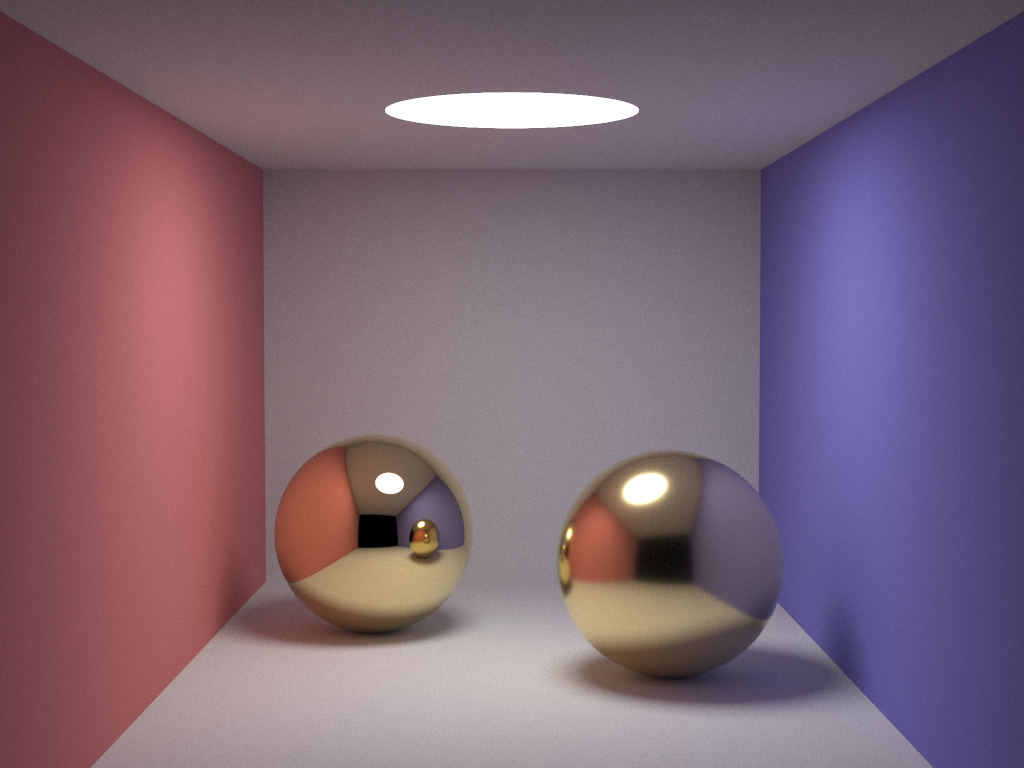
\includegraphics[width=0.5\textwidth]{convergedIS.png}
    \caption{converged final image}
\end{figure}

\begin{figure}
\centering
\begin{subfigure}{.5\textwidth}
  \centering
  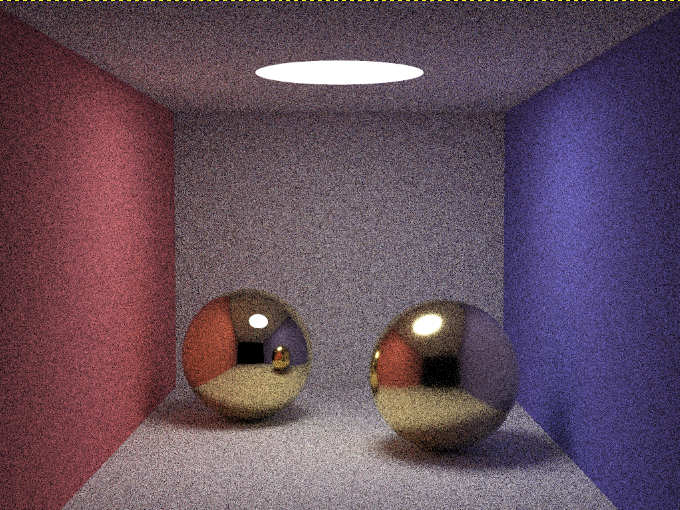
\includegraphics[width=.9\linewidth]{IS100.png}
  \caption{Importance sampling, 100 samples}
  \label{fig:sub1}
\end{subfigure}%
\begin{subfigure}{.5\textwidth}
  \centering
  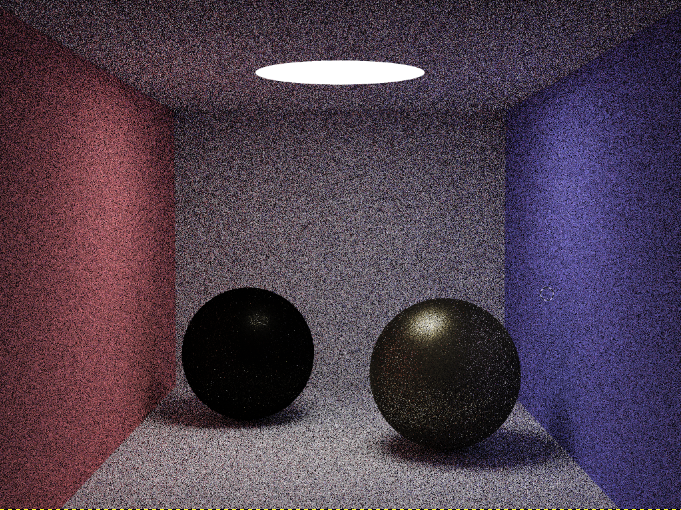
\includegraphics[width=.9\linewidth]{DS100.png}
  \caption{Direct sampling, 100 samples}
  \label{fig:sub2}
\end{subfigure}
\begin{subfigure}{.5\textwidth}
  \centering
  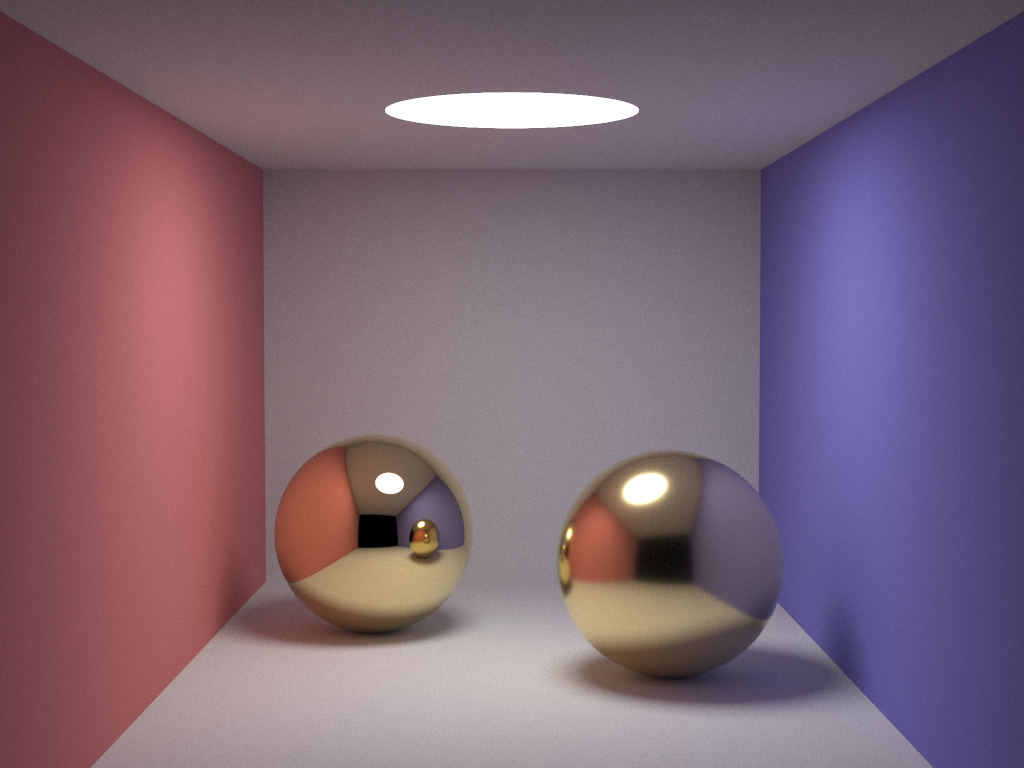
\includegraphics[width=.9\linewidth]{convergedIS.png}
  \caption{Importance sampling, 10,0000 samples}
  \label{fig:sub1}
\end{subfigure}%
\begin{subfigure}{.5\textwidth}
  \centering
  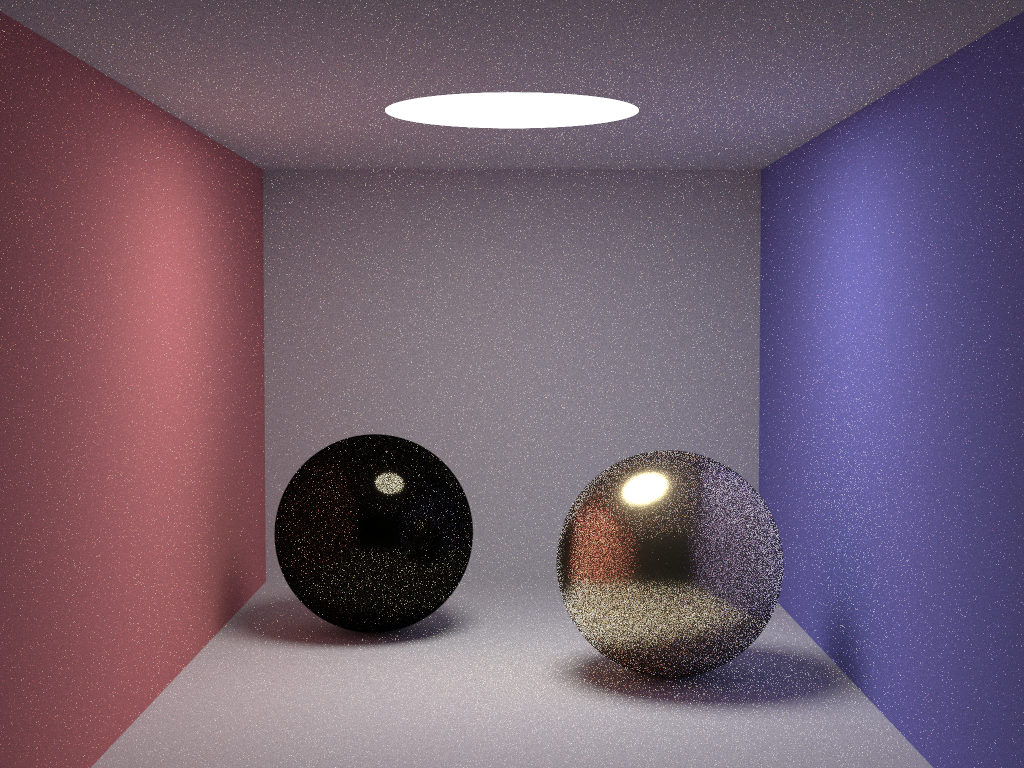
\includegraphics[width=.9\linewidth]{10KDS.png}
  \caption{Direct sampling, 10,000 samples}
  \label{fig:sub1}
\end{subfigure}%
\caption{render with and without importance sampling}
\label{fig:test}
\end{figure}

\noindent In order to quantitatively demonstrate the convergence rate between using direct and importance sampling techniques, we collected a sequence of images rendered under different number of samples for both cases. Since each image is comprised of a $768\times 1024$ matrix where every pixel stores a RGB value, by calculating the Mean Square Root Error $\alpha$ = $|$ Tn - I $|$ of every matrix in the sequence of the rendered images, where Tn is the converged matrix and I is the matrix generated at a given number of samples, we can plot the absolute Error versus the number of samples. Figure 4 shows the change in $\alpha_n$ as the number of samples increases in the case of using direct sampling, and figure 5 shows the case where importance sampling techniques are used.

\begin{figure}[H]
  \centering
    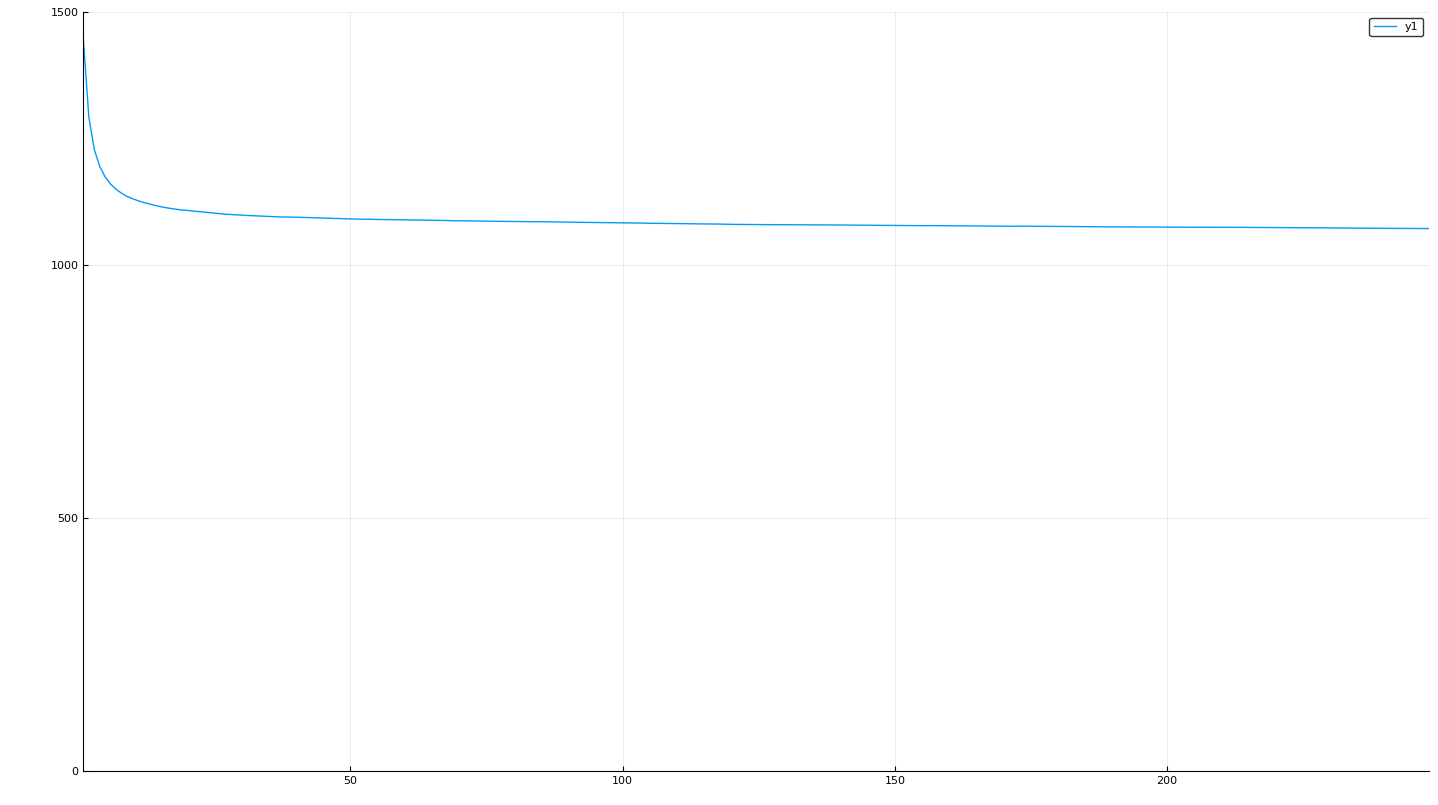
\includegraphics[width=0.9\textwidth]{DS1000.png}
    \caption{Direct sampling, 1000 samples}
\end{figure}

\begin{figure}[H]
  \centering
    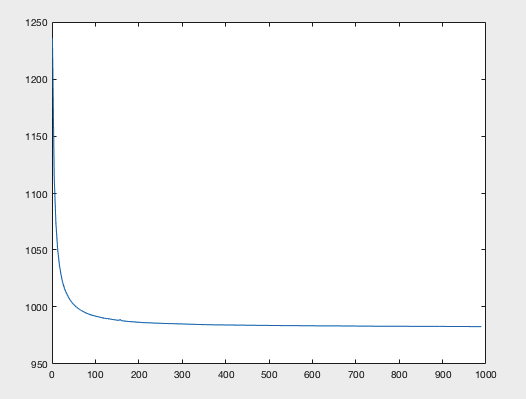
\includegraphics[width=0.9\textwidth]{IS1000.png}
    \caption{Importance sampling, 1000 samples}
\end{figure}

In figure 4, the value of the absolute error after 1000 samples is about 1100, suggesting that for this rendering to converge, it will require a significantly larger number of samples. On the other hand, when importance sampling techniques are used in the rendering, by the time of 1000 samples, the value of absolute error is about 980. 
Although this difference may not seem numerically significant, the visual implications of this difference are quite stark.

We hypothesize that the failure of the importance sampled algorithm to converge was due to a mistake in luminance clamping on our part. 
We intend to address this issue in the future.

\section{Discussion}

We can see that in the case where the BSDF approaches a Dirac delta, a surface without importance sampling may never converge within a reasonable number of samples.
As a result importance sampling is absolutely essential for raytracing in a practical setting.
Fortunately, most BSDF are designed to yield fast importance samplers, so it is both mathematically practical and computationally inexpensive to implement importance sampling. 

\end{document}
